
%%%%%%%%%%%%%%%%%%%%%%%%%%%%%%%%%%%%%%%%%%%%%%%%%%%%%%%%%%%%%%%%%%%%%%%%%%%%%%%%
%%%%%%%%%%% Document class and package options
%%%%%%%%%%%%%%%%%%%%%%%%%%%%%%%%%%%%%%%%%%%%%%%%%%%%%%%%%%%%%%%%%%%%%%%%%%%%%%%%
% \documentclass[a4paper,12pt]{article}
\documentclass[a4paper,12pt,twoside]{article}
\usepackage{outline}

\usepackage{amsmath}
\usepackage{amssymb}                    % AMS Math
\usepackage{amsfonts}
\usepackage[tight,hang,centerlast]{subfigure}
\usepackage[lined,ruled,longend]{algorithm2e}

\clubpenalty=1000
\widowpenalty=1000

%% eps to pdf
%% specify .eps extension when \includegraphics if you want the .pdf fig file to
%%     be regenerated as part of the compilation. Without extension the .pdf fig
%%     file is generated only if it does not exist yet
%% --shell-escape option must be enabled
\newif\ifpdf
\ifx\pdfoutput\undefined
   \pdffalse
\else
   \pdfoutput=1
   \pdftrue
\fi
\ifpdf
   \usepackage{graphicx}
   \usepackage{epstopdf}

   \epstopdfsetup{suffix=}

   \DeclareGraphicsRule{.eps}{pdf}{.pdf}{`epstopdf #1}
   \pdfcompresslevel=9
\else
   \usepackage{graphicx}
\fi


\begin{document}


%%%%%%%%%%%%%%%%%%%%%%%%%%%%%%%%%%%%%%%%%%%%%%%%%%%%%%%%%%%%%%%%%%%%%%%%%%%%%%%%
%%%%%%%%%%% Title
%%%%%%%%%%%%%%%%%%%%%%%%%%%%%%%%%%%%%%%%%%%%%%%%%%%%%%%%%%%%%%%%%%%%%%%%%%%%%%%%

\title{Measurement Results from\\
Wireless Battle Mesh\\
Version 6}


%\date{April, 2013}

\contributors{WBM community}
\eventlocation{Aalborg University. Aalborg, Denmark}
\eventdates{15th to 21st of April 2013}
\eventurl{http://battlemesh.org/BattleMeshV6}
\doctype{measurement report}
\logofigure{figures/battlemeshv6}

\frontmatter

\maketitle

%%%%%%%%%%%%%%%%%%%%%%%%%%%%%%%%%%%%%%%%%%%%%%%%%%%%%%%%%%%%%%%%%%%%%%%%%%%%%%%%
%%%%%%%%%%% Indices
%%%%%%%%%%%%%%%%%%%%%%%%%%%%%%%%%%%%%%%%%%%%%%%%%%%%%%%%%%%%%%%%%%%%%%%%%%%%%%%%

\thispagestyle{plain}
%\vspace*{3cm}

%\begin{center}
%\LARGE{\textbf{Abstract}} 
%\end{center}

%\begin{itemize}
%\item TODO..
%\end{itemize}

%\cleardoublepage
\clearsinglepage

\thispagestyle{plain}
\tableofcontents

%\cleardoublepage
\clearsinglepage

%%%%%%%%%%%%%%%%%%%%%%%%%%%%%%%%%%%%%%%%%%%%%%%%%%%%%%%%%%%%%%%%%%%%%%%%%%%%%%%%
%%%%%%%%%%% The document
%%%%%%%%%%%%%%%%%%%%%%%%%%%%%%%%%%%%%%%%%%%%%%%%%%%%%%%%%%%%%%%%%%%%%%%%%%%%%%%%

\singlespacing
\mainmatter
%%%%%%%%%%%%%%%%%%%%%%%%%%%%%%%%%%%%%%%%%%%%%%%%%%%%%%%%%%%%%%%%%%%%%%%%%%%%%%%%
%%%%%%%%%%% Chapter Inclusion
%%%%%%%%%%%%%%%%%%%%%%%%%%%%%%%%%%%%%%%%%%%%%%%%%%%%%%%%%%%%%%%%%%%%%%%%%%%%%%%%


%%%%%%%%%%%%%%%%%%%%%%%%%%%%%%%%%%%%%%%%%%%%%%%%%%%%%%%%%%%%%%%%%%%%%%%%%%%%%%%%
%%%%%%%%%%%%%%%%%%%%%%%%%%%%%%%%%%%%%%%%%%%%%%%%%%%%%%%%%%%%%%%%%%%%%%%%%%%%%%%%
\thispagestyle{plain}

%%%%%%%%%%%%%%%%%%%%%%%%%%%%%%%%%%%%%%%%%%%%%%%%%%%%%%%%%%%%%%%%%%%%%%%%%%%%%%%%
%%%%%%%%%%%%%%%%%%%%%%%%%%%%%%%%%%%%%%%%%%%%%%%%%%%%%%%%%%%%%%%%%%%%%%%%%%%%%%%%
%%%%%%%%%%%%%%%%%%%%%%%%%%%%%%%%%%%%%%%%%%%%%%%%%%%%%%%%%%%%%%%%%%%%%%%%%%%%%%%%
\section{Introduction}
\label{sec:introduction}


WBM...

%%%%%%%%%%%%%%%%%%%%%%%%%%%%%%%%%%%%%%%%%%%%%%%%%%%%%%%%%%%%%%%%%%%%%%%%%%%%%%%%
%%%%%%%%%%%%%%%%%%%%%%%%%%%%%%%%%%%%%%%%%%%%%%%%%%%%%%%%%%%%%%%%%%%%%%%%%%%%%%%%
%%%%%%%%%%%%%%%%%%%%%%%%%%%%%%%%%%%%%%%%%%%%%%%%%%%%%%%%%%%%%%%%%%%%%%%%%%%%%%%%
\section{Protocols}


\subsection{Babel}

\subsection{Batman-adv}

\subsection{Bmx6}

\subsection{OLSR}


%%%%%%%%%%%%%%%%%%%%%%%%%%%%%%%%%%%%%%%%%%%%%%%%%%%%%%%%%%%%%%%%%%%%%%%%%%%%%%%%
%%%%%%%%%%%%%%%%%%%%%%%%%%%%%%%%%%%%%%%%%%%%%%%%%%%%%%%%%%%%%%%%%%%%%%%%%%%%%%%%
%%%%%%%%%%%%%%%%%%%%%%%%%%%%%%%%%%%%%%%%%%%%%%%%%%%%%%%%%%%%%%%%%%%%%%%%%%%%%%%%
\section{Testbed Descripiton}

\subsection{Node System}

\subsection{Topology}

% wget http://downloads.battlemesh.org/WBMv6/geographical_map1.png
% wget http://downloads.battlemesh.org/WBMv6/geographical_map2.png
\begin{figure}[!ht]
\centering
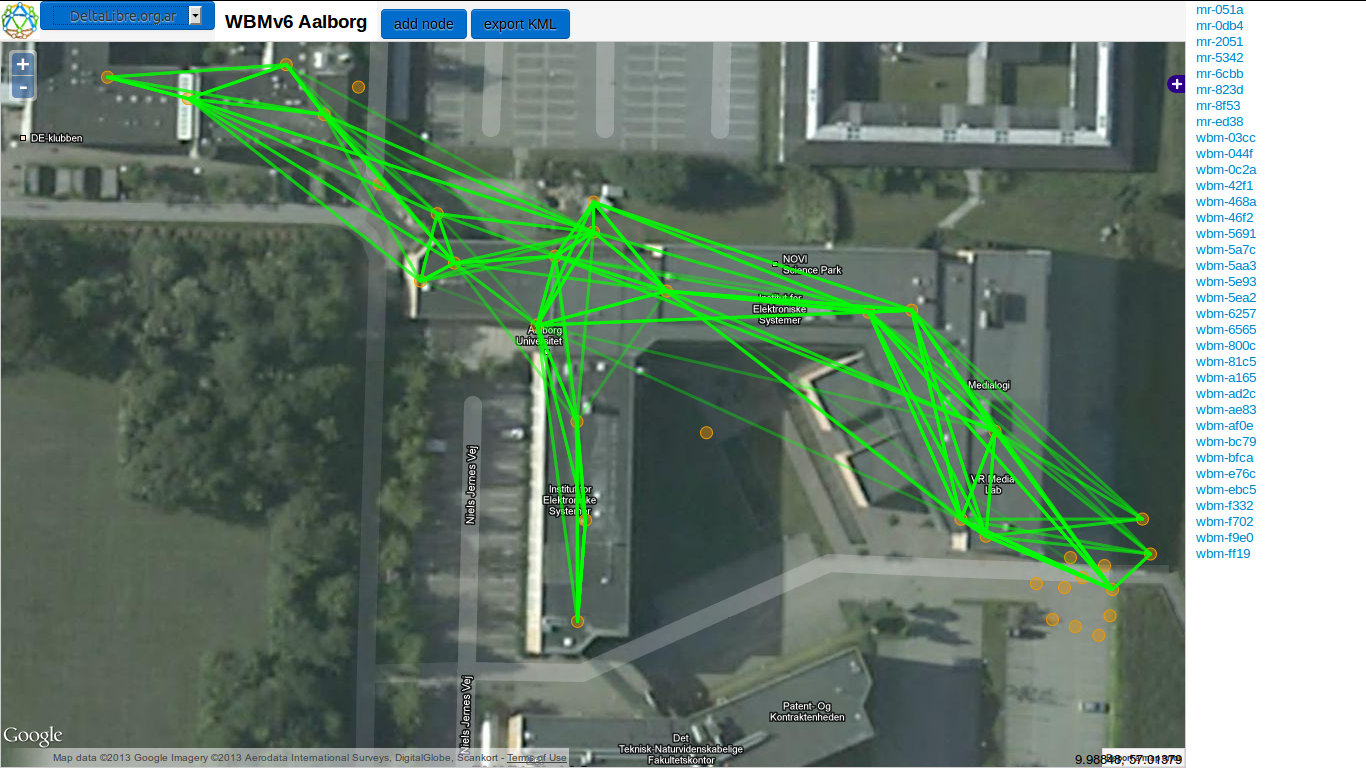
\includegraphics[width=1.4\textwidth, angle=90]{figures/geographical_map2.png}
\caption{geographical map snapshot}
\label{fig:geomap}
\end{figure}


% wget -O topo0.svg "http://battlemesh.org/BattleMeshV6/Tests?action=AttachFile&do=get&target=topo0.svg"
% \immediate\write18{ inkscape -D -z --file=topo0.svg --export-pdf=topo0.pdf }

\begin{figure}[!ht]
\centering
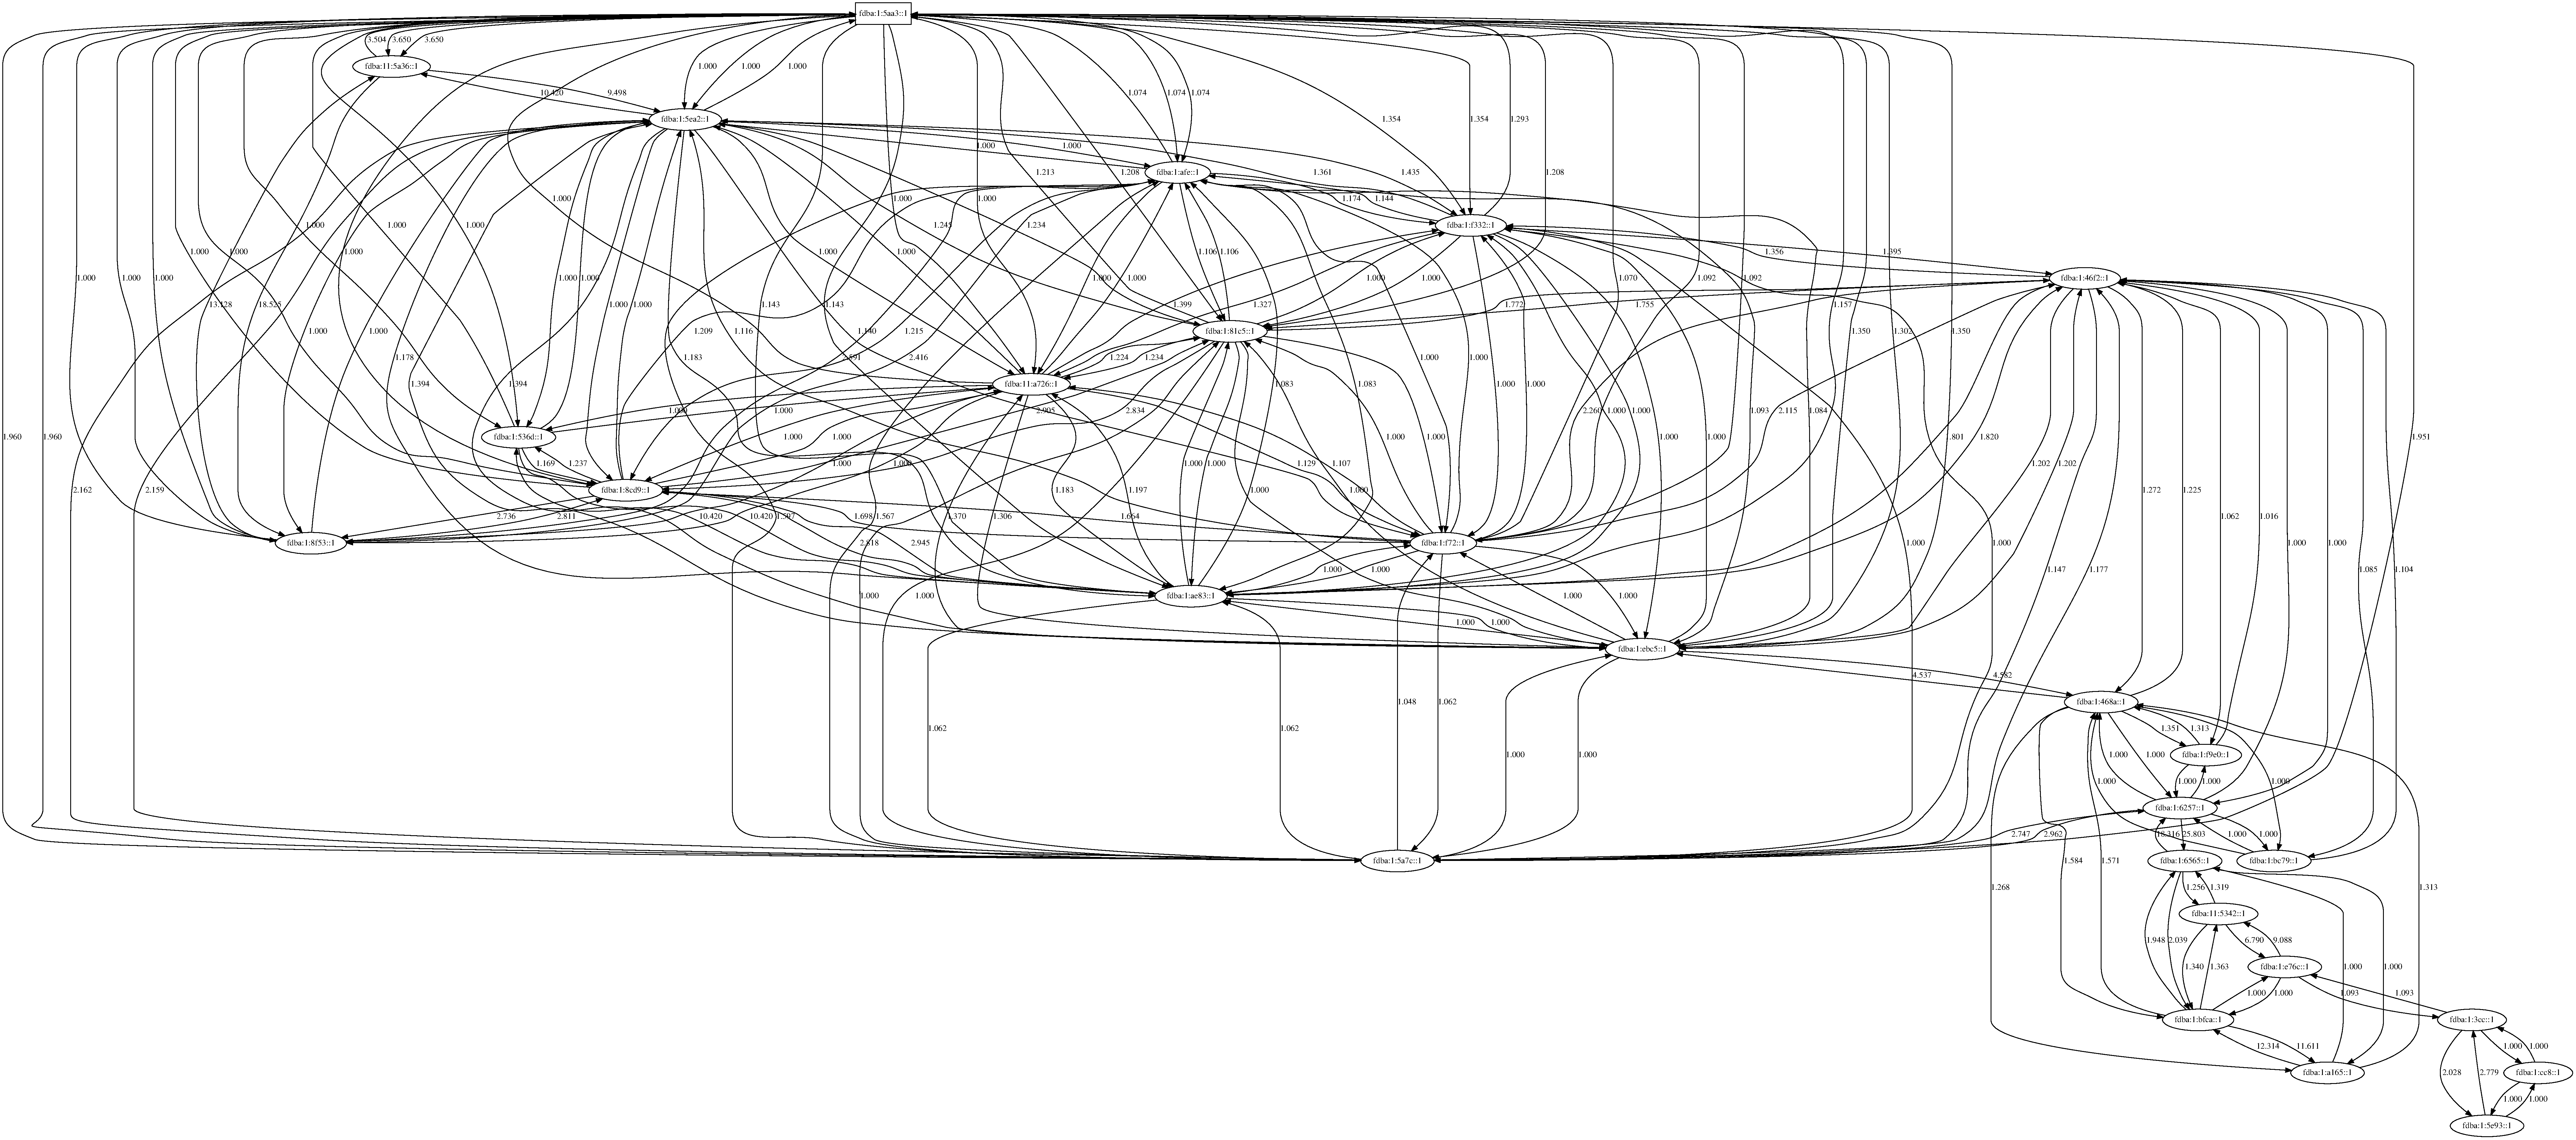
\includegraphics[width=1.4\textwidth, angle=90]{figures/topo0.pdf}
\caption{OLSR topology snapshot}
\label{fig:olsr-topo}
\end{figure}

%\begin{figure}[h]
%\centering
%\def\svgwidth{\columnwidth}
%\includesvg{topo0}
%\end{figure}


%%%%%%%%%%%%%%%%%%%%%%%%%%%%%%%%%%%%%%%%%%%%%%%%%%%%%%%%%%%%%%%%%%%%%%%%%%%%%%%%
%%%%%%%%%%%%%%%%%%%%%%%%%%%%%%%%%%%%%%%%%%%%%%%%%%%%%%%%%%%%%%%%%%%%%%%%%%%%%%%%
%%%%%%%%%%%%%%%%%%%%%%%%%%%%%%%%%%%%%%%%%%%%%%%%%%%%%%%%%%%%%%%%%%%%%%%%%%%%%%%%
\section{Ping Measurements (hops, rtt, loss)}
\label{sec:ping-measurements}

%%%%%%%%%%%%%%%%%%%%%%%%%%%%%%%%%%%%%%%%%%%%%%%%%%%%%%%%%%%%%%%%%%%%%%%%%%%%%%%%
\subsection{Assumptions}



%%%%%%%%%%%%%%%%%%%%%%%%%%%%%%%%%%%%%%%%%%%%%%%%%%%%%%%%%%%%%%%%%%%%%%%%%%%%%%%%
%\immediate\write18{ ../eval.R --data=../tmp.data --stat=../tmp.stat --imgdir=../img --texdir=inputs/ }

%%%%%%%%%%%%%%%%%%%%%%%%%%%%%%%%%%%%%%%%%%%%%%%%%%%%%%%%%%%%%%%%%%%%%%%%%%%%%%%%
\subsection{Stationary Scenarios}

\makeFigure{sArtt}{Random node test 1}{0.7}
\makeFigure{sArvh}{Random node test 1}{0.7}
\makeFigure{sBrtt}{Random node test 2}{0.7}
\makeFigure{sBrvh}{Random node test 2}{0.7}

\makeCCTabl{tbl:s4-s6}{Individual Random node tests (groups 4-6)} {%
      \makeGraphic{s4rtt} & \makeGraphic{s4rvh} \\
      \makeGraphic{s5rtt} & \makeGraphic{s5rvh} \\
      \makeGraphic{s6rtt} & \makeGraphic{s6rvh} \\
}

\makeCCTabl{tbl:s7-s9}{Individual Random node tests (groups 7-9)} {%
      \makeGraphic{s7rtt} & \makeGraphic{s7rvh} \\
      \makeGraphic{s8rtt} & \makeGraphic{s8rvh} \\
      \makeGraphic{s9rtt} & \makeGraphic{s9rvh} \\
}

\makeCCTabl{tbl:s10-s12}{Individual Random node tests (groups 10-12)} {%
      \makeGraphic{s10rtt} & \makeGraphic{s10rvh} \\
      \makeGraphic{s11rtt} & \makeGraphic{s11rvh} \\
      \makeGraphic{s12rtt} & \makeGraphic{s12rvh} \\
}

\makeCCTabl{tbl:s13-s15}{Individual Random node tests (groups 13-15)} {%
      \makeGraphic{s13rtt} & \makeGraphic{s13rvh} \\
      \makeGraphic{s14rtt} & \makeGraphic{s14rvh} \\
      \makeGraphic{s15rtt} & \makeGraphic{s15rvh} \\
}

\makeCCTabl{tbl:s16-s18}{Individual Random node tests (groups 16-18)} {%
      \makeGraphic{s16rtt} & \makeGraphic{s16rvh} \\
      \makeGraphic{s17rtt} & \makeGraphic{s17rvh} \\
      \makeGraphic{s18rtt} & \makeGraphic{s18rvh} \\
}

\makeCCTabl{tbl:s19-s21}{Individual Random node tests (groups 19-21)} {%
      \makeGraphic{s19rtt} & \makeGraphic{s19rvh} \\
      \makeGraphic{s20rtt} & \makeGraphic{s20rvh} \\
      \makeGraphic{s21rtt} & \makeGraphic{s21rvh} \\
}


\makeCCTabl{tbl:s22-s24}{Individual Random node tests (groups 22-24)} {%
      \makeGraphic{s22rtt} & \makeGraphic{s22rvh} \\
      \makeGraphic{s23rtt} & \makeGraphic{s23rvh} \\
      \makeGraphic{s24rtt} & \makeGraphic{s24rvh} \\
}

\makeCCTabl{tbl:s25-s27}{Individual Random node tests (groups 25-27)} {%
      \makeGraphic{s25rtt} & \makeGraphic{s25rvh} \\
      \makeGraphic{s26rtt} & \makeGraphic{s26rvh} \\
      \makeGraphic{s27rtt} & \makeGraphic{s27rvh} \\
}

\makeCCTabl{tbl:s28}{Individual Random node tests (group 28)} {%
      \makeGraphic{s28rtt} & \makeGraphic{s28rvh} \\
}

%%%%%%%%%%%%%%%%%%%%%%%%%%%%%%%%%%%%%%%%%%%%%%%%%%%%%%%%%%%%%%%%%%%%%%%%%%%%%%%%
\subsection{Mobile Scenarios}

\makeCCTabl{tbl:m0-m2}{Individual mobile and running node scenarios} {%
      \makeGraphic{m0rtt} & \makeGraphic{m0tim} \\
      \makeGraphic{m0hop} & \makeGraphic{m0rvh} \\

}

%\makeCCTabl{tbl:m0-m2}{Individual mobile and running node scenarios} {%
%      \makeGraphic{m0rtt} & \makeGraphic{m0tim} \\
%      \makeGraphic{m1rtt} & \makeGraphic{m1tim} \\
%      \makeGraphic{m2rtt} & \makeGraphic{m2tim} \\
%}


%\begin{figure}
% \centering
% \includegraphics[width=1\textwidth]{../img/out.pdf}
% \caption{Research guidelines}
% \label{fig:guidelines}
%\end{figure}


%%%%%%%%%%%%%%%%%%%%%%%%%%%%%%%%%%%%%%%%%%%%%%%%%%%%%%%%%%%%%%%%%%%%%%%%%%%%%%%%
%%%%%%%%%%%%%%%%%%%%%%%%%%%%%%%%%%%%%%%%%%%%%%%%%%%%%%%%%%%%%%%%%%%%%%%%%%%%%%%%
%%%%%%%%%%%%%%%%%%%%%%%%%%%%%%%%%%%%%%%%%%%%%%%%%%%%%%%%%%%%%%%%%%%%%%%%%%%%%%%%
\section{TCP Throughput Measurements}
\label{sec:tp-measurements}


%%%%%%%%%%%%%%%%%%%%%%%%%%%%%%%%%%%%%%%%%%%%%%%%%%%%%%%%%%%%%%%%%%%%%%%%%%%%%%%%
%%%%%%%%%%%%%%%%%%%%%%%%%%%%%%%%%%%%%%%%%%%%%%%%%%%%%%%%%%%%%%%%%%%%%%%%%%%%%%%%
%%%%%%%%%%%%%%%%%%%%%%%%%%%%%%%%%%%%%%%%%%%%%%%%%%%%%%%%%%%%%%%%%%%%%%%%%%%%%%%%
\section{Appendix}



%%%%%%%%%%%%%%%%%%%%%%%%%%%%%%%%%%%%%%%%%%%%%%%%%%%%%%%%%%%%%%%%%%%%%%%%%%%%%%%%
%%%%%%%%%%%%%%%%%%%%%%%%%%%%%%%%%%%%%%%%%%%%%%%%%%%%%%%%%%%%%%%%%%%%%%%%%%%%%%%%
%\section*{Acknowledgements}
%
%This work is supported by ...


%%%%%%%%%%%%%%%%%%%%%%%%%%%%%%%%%%%%%%%%%%%%%%%%%%%%%%%%%%%%%%%%%%%%%%%%%%%%%%%%
%%%%%%%%%%%%%%%%%%%%%%%%%%%%%%%%%%%%%%%%%%%%%%%%%%%%%%%%%%%%%%%%%%%%%%%%%%%%%%%%

\backmatter

\bibliographystyle{ieeetr}
%\bibliography{biblio-data}

\end{document} 
